% document class
\documentclass{scrartcl}

% encoding
\usepackage[T1]{fontenc}
\usepackage[utf8]{inputenc}%utf8

% language
\usepackage[ngerman]{babel}
\usepackage{scrhack} % nach \documentclass
\usepackage[aux]{rerunfilecheck}
\usepackage{polyglossia}
\setmainlanguage{german}

% math
\usepackage{amsmath}
\usepackage{amsfonts}
\usepackage{amssymb}
\usepackage{amstext}
\usepackage{isomath}
\usepackage{mathtools}

% physics
\usepackage{tensor}
\usepackage{slashed}
\usepackage{braket}
\usepackage[strict, separate-uncertainty, sticky-per]{siunitx}

% fonts
\usepackage{microtype}
\usepackage{fourier}
\usepackage{tgheros}
\usepackage{tgcursor}
\usepackage{tgpagella}

% tikz
\usepackage{tikz}

% margins
\usepackage[top=2.5cm]{geometry}

% variables
\newcommand{\thehandover}{Freitag, den 20.\,Oktober 2017 12:00 Uhr}
\newcommand{\thesheet}{1}
\newcommand{\thesemester}{WS 17/18}
\newcommand{\theprofessor}{Priv.-Doz.~U.~Löw}

% enumeration
\renewcommand{\labelenumi}{(\alph{enumi})} % alphabetic tasks
\renewcommand{\theenumi}{(\alph{enumi})} % alphabetic tasks
\usepackage{enumitem} % allows to continue lists with [resume]

% clickable links and '\url' command
\usepackage[hidelinks]{hyperref}

\usepackage{placeins}



\newcommand{\ua}[1]{_\symup{#1}}
\newcommand{\su}[1]{\symup{#1}}


\newcounter{exercise}
\newenvironment{exercise}
[2]
{\addtocounter{exercise}{1}{\bfseries{Aufgabe \arabic{exercise}:~#1}\hfill(#2 Punkte)}\newline}
{\medskip}

\setlength{\parindent}{0mm}
\begin{document}
{\large\bfseries 6. Übungsblatt zur Vorlesung\hfill\thesemester}\\ %/thesheet
{\large\bfseries Theoretische Physik I\hfill\theprofessor}\\
%{\large\bfseries Abgabe: bis \thehandover}\\
{\large\bfseries Abgabe bis: 24.11.}\\
\textbf{Webseite zur Vorlesung: \\}
\url{https://moodle.tu-dortmund.de/course/view.php?id=9519} \\
\rule{\columnwidth}{0.1ex}
\medskip

\begin{exercise}{Teilchen im Kegelmantel}{10}


  \begin{enumerate}
    \item[a)] Überlegen Sie sich die vorhandenen Zwangsbedingungen, wenn sich ein
    Teilchen auf einem Kegelmantel bewegt (Abbildung \ref{fig:TiK}).
    Formulieren Sie die Zwangsbedingung
    so um, dass $\Phi(r,z) = 0$ gilt. Wie viele Freiheitsgrade existieren
    in diesem System anschlie\ss{}end noch?

    \FloatBarrier
    \begin{figure}
      \centering
      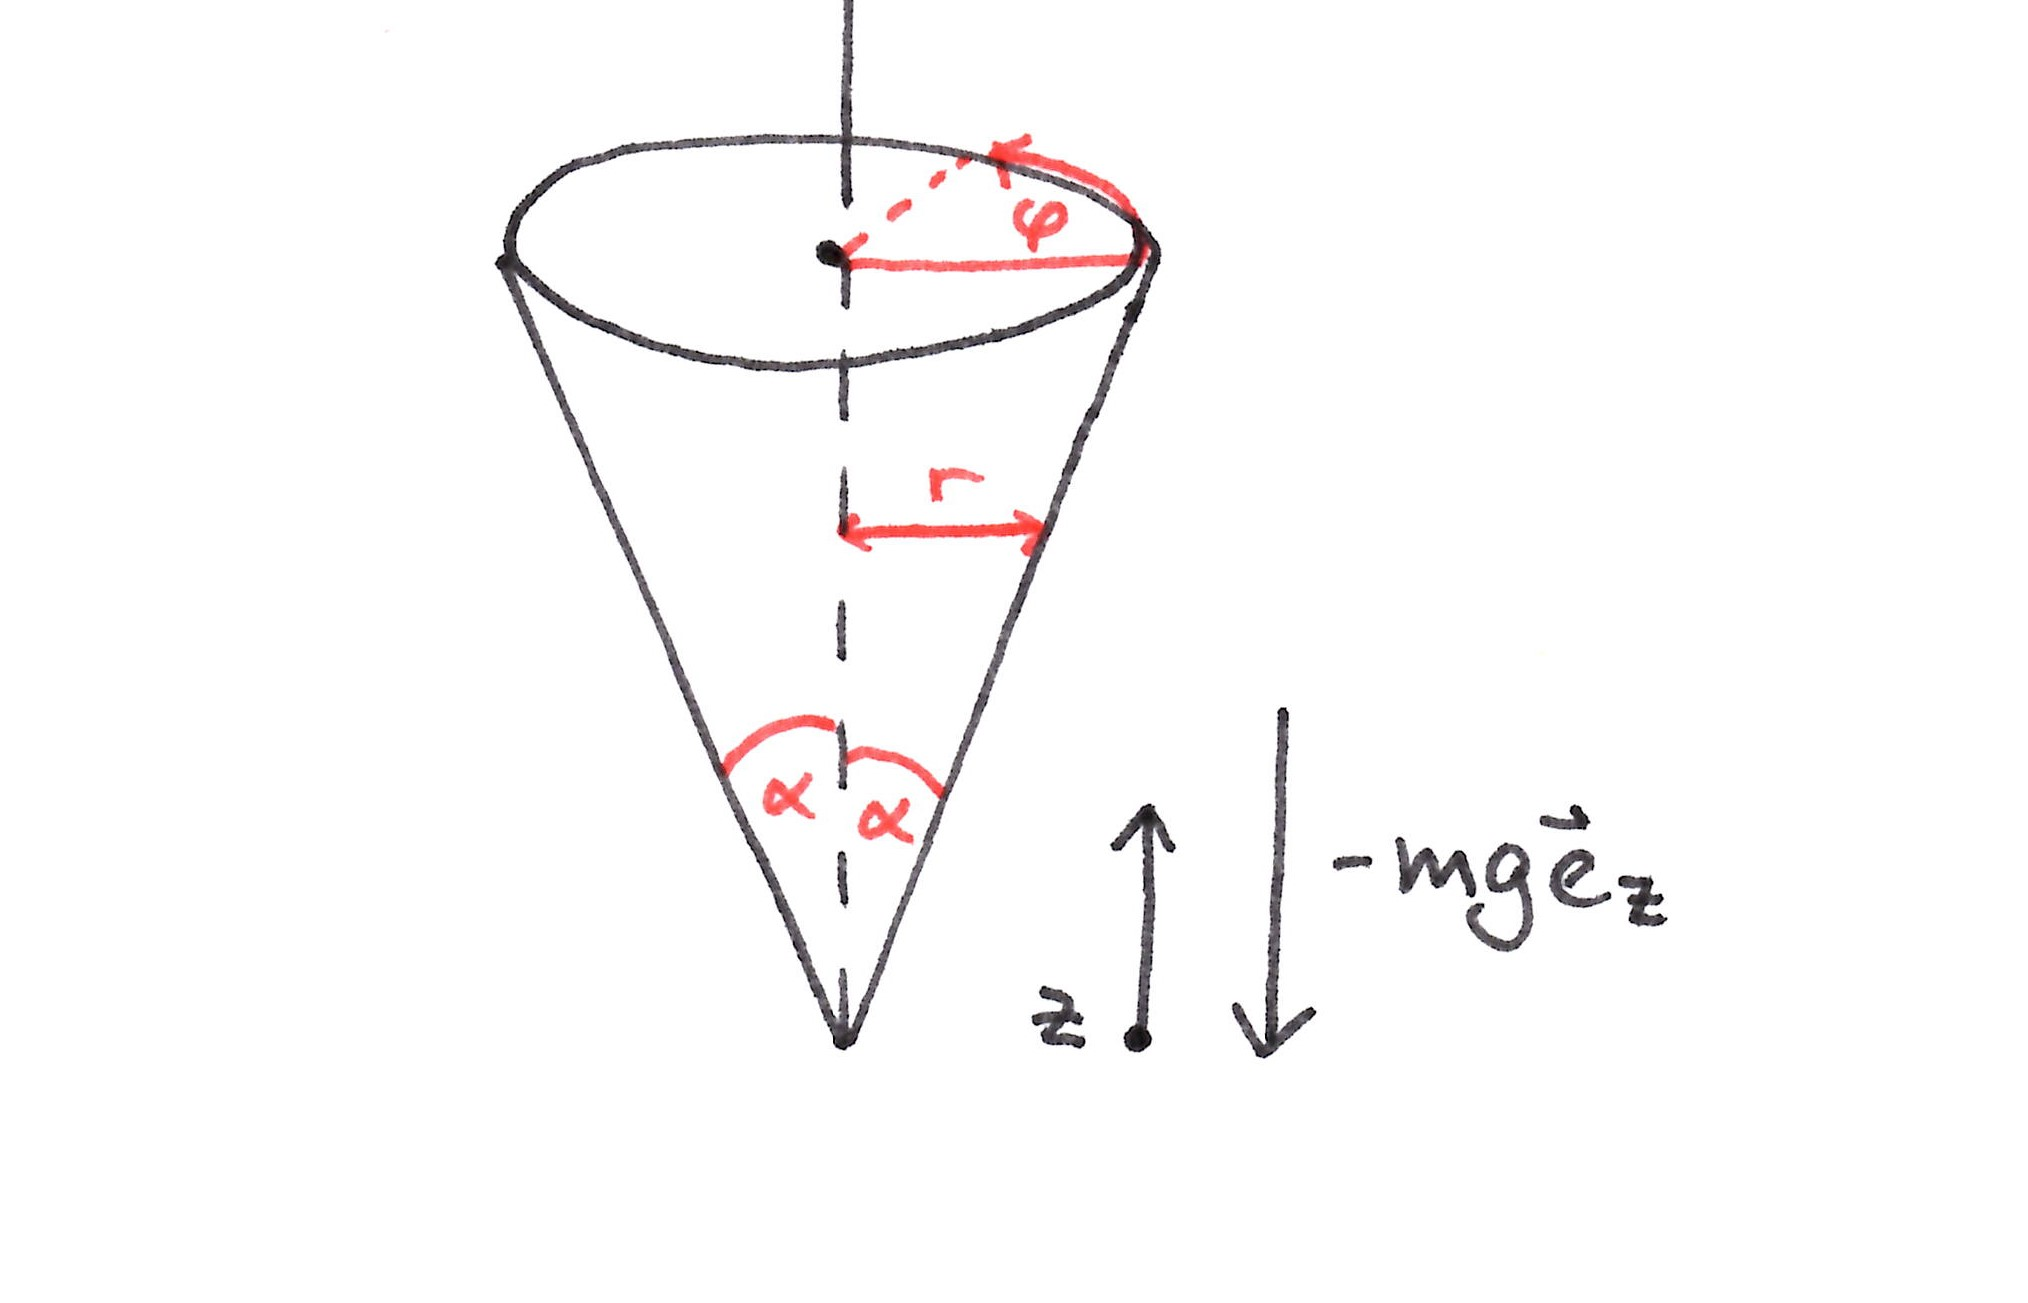
\includegraphics[width = 7 cm]{Kegel.jpg}
      \caption{Teilchen im Kegelmantel.}
      \label{fig:TiK}
    \end{figure}

    \item[\bullet]Durch jede Zwangsbedingung wird die Anzahl der Freiheitsgrade in einem System
    verringert. Um diese Zwangsbedingung zu berücksichtigen, wird die Zwangskraft
    eingeführt, welche dafür sorgt, dass das Teilchen eine reduzierte Bewegung
    ausführt. Um die Richtung der Zwangskräfte zu bestimmen, wird dabei
    die Relation $ \vec{\nabla} \Phi \parallel \vec{Z}$ verwendet. Für die
    Zwangskraft wird dann der Betrag $-\lambda$ angenommen, so dass sich

    \begin{equation}
      \vec{Z} = - \lambda \vec{\nabla} \Phi
    \end{equation}

    ergibt. Die Zwangskraft ist die Kraft, die dafür sorgt dass sich das Teilchen
    auf dem Zylindermantel bewegt, steht also senkrecht auf diesen. Wieso ist
    somit auch die Annahme $ \vec{\nabla} \Phi \parallel \vec{Z}$ gerechtfertigt?

    \item[b)] Bestimmen Sie $\vec{Z}$, indem Sie ein geeignetes Koordinatensystem
    verwenden und die oben genannten Relationen verwenden.

    \item[\bullet]In dem am besten geeigneten Koordinatensystem gilt für die Beschleunigung

    \begin{equation}
      \ddot{\vec{r}} = ( \ddot{r}-r\dot{\varphi}^2)\vec{e}_{r} + (r\ddot{\varphi}
      + 2\dot{r}\dot{\varphi})\vec{e}_{\varphi} + \ddot{z}\vec{e}_{z}.
      \label{eqn:Geschw}
    \end{equation}

    Die Newtonsche Bewegungsgleichung lautet für dieses System :

    \begin{equation}
      m \ddot{\vec{r}} = - mg\vec{e}_{z} + \vec{Z}.
      \label{eqn:Newton}
    \end{equation}

    \item[c)] Stellen Sie die Newtonsche Bewegungsgleichung auf, indem Sie
    \eqref{eqn:Geschw} sowie Ihr bestimmtes $\vec{Z}$ in \eqref{eqn:Newton}
    einsetzen. Durch einen Koeffizientenvergleich bezüglich der Terme vor den
    Einheitsvektoren lassen sich 3 Gleichungen formulieren.

    Unter Hinzunahme der
    Zwangsbedingung lassen sich mittels 3 der 4 Gleichungen $\lambda$ und $z$
    eliminieren. Stellen Sie anhand der dann erhaltenden 2 Bewegungsgleichungen
    eine Vermutung auf, welche physikalische Grö\ss{}e in diesem System erhalten ist.
    \\
    \textit{Hinweis: $r\ddot{\varphi} + 2\dot{r}\dot{\varphi} = 0$ wird zum Eliminieren
    von $\lambda$ und $z$ nicht benötigt}

    \item[d)] Betrachten Sie das Problem nun mittels der Euler-Lagrange-Gleichung.
    Überlegen Sie sich, welche zwei generalisierten Koordinaten zu wählen sind
    (siehe vorherige Teilaufgaben) und stellen sie die Lagrange-Funktion auf.

    \item[e)] Ermitteln Sie nun mittels der Euler-Lagrange-Gleichung die Bewegungsgleichungen
    des Systems. Überlegen und Begründen Sie, welche physikalische Grö\ss{}e erhalten
    ist. Wie kann die Erhaltungsgrö\ss{}e auch anhand der Lagrange-Funktion erkannt
    werden? (Begründung anhand der Euler-Lagrange-Gleichung). Welche Auswirkung
    hat die Erhaltungsgrö\ss{}e auf die Bewegung des Teilchens im Kegelmantel?

  \end{enumerate}
\end{exercise}

\begin{exercise}{Perle auf Draht}{10}
  Betrachten Sie eine Perle auf einem Draht. Die Perle besitzt die Masse $m$
  und gleitet reibungsfrei auf einem Draht, welcher durch die Funktion $z = h(x)$
  beschrieben wird.

  \begin{figure}[h]
    \centering
    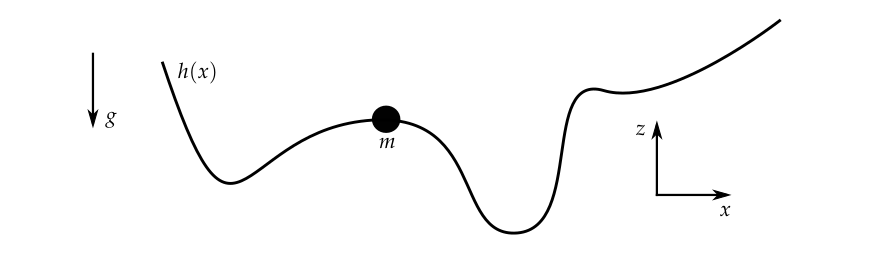
\includegraphics[width=\textwidth]{Blatt_06_PerleaufDraht.png}
    \label{fig:Höhenprofil}
  \end{figure}

    \begin{enumerate}
        \item Bestimmen Sie für einen beliebig geformten Draht $h(x)$ die Lagrange-Funktion
        in der generalisierten Koordinate $x$.
        \item Nutzen Sie die Euler-Lagrange-Gleichung, um die Bewegungsgleichung
        des Massepunktes aufzustellen.
        \item Setzen Sie nun die folgenden Funktionen $h(x)$ in die Bewegungsgleichung
        ein:
        \begin{itemize}
          \item[(i)] Welche Bewegung wird für $h(x) = h_0$ angenommen?
          \item[(ii)] $h(x) = ax$. Zeigen Sie anhand der Bewegungsgleichung, dass
          auf die Perle nur die konstante Hangabtriebskraft
          \begin{equation}
            \label{eqn:Hangabtrieb}
            \left|\vec{F}_{H}\right| = mg\sin\left(\alpha\right)
          \end{equation}
          wirkt, wobei $\alpha$ den Steigungswinkel der Funktion, d.h. den Winkel
          zwischen Funktionsgraph und der $x$-Achse, bezeichnet.
          \item[(iii)] Sei nun $h(x) = \frac{b}{2}x^2$. Die Bewegungsgleichung enthält
           neben der Hangabtriebskraft einen weiteren Term. Welche Kraft beschreibt
           dieser?\\

           Welche Form nimmt die Bewegungsgleichung für $b > 0$ an, wenn die
           Auslenkungen $x$
           und die Geschwindigkeiten $\dot{x}$ so klein sind, dass nur die linearen Terme
           berücksichtigt werden müssen?\\
         \end{itemize}
           \item Berechnen Sie aus der Lagrange-Funktion, die Sie in Aufgabenteil (a)
           bestimmt haben, die Erhaltungsgrö\ss e

    \begin{equation}
      \label{eqn:Hamilton}
      H = \dot{x}\frac{\partial L}{\partial\dot{x}} - L.
    \end{equation}
    Um welche Grö\ss e handelt es sich hierbei?
    \end{enumerate}
\end{exercise}

\end{document}
